%%%%%%%%%%%%%%%%%%%%%%%%%%%%%%%%%%%%
% Slide options
%%%%%%%%%%%%%%%%%%%%%%%%%%%%%%%%%%%%

% Option 1: Slides with solutions

\documentclass[slidestop,compress,mathserif]{beamer}
\newcommand{\soln}[1]{\textit{#1}}
\newcommand{\solnGr}[1]{#1}

% Option 2: Handouts without solutions

%\documentclass[11pt,containsverbatim,handout]{beamer}
%\usepackage{pgfpages}
%\pgfpagesuselayout{4 on 1}[letterpaper,landscape,border shrink=5mm]
%\newcommand{\soln}[1]{ }
%\newcommand{\solnGr}{ }

%%%%%%%%%%%%%%%%%%%%%%%%%%%%%%%%%%%%
% Style
%%%%%%%%%%%%%%%%%%%%%%%%%%%%%%%%%%%%

\usetheme{AnnArbor}

% Load color theme: There are a variety of color themes available, not limited to the ones listed below. Make sure to use only one at a time and comment out the rest.
%\usecolortheme{albatross}
%\usecolortheme{dolphin}
\usecolortheme{seahorse}
%\usecolortheme{seagull}

\usepackage{geometry}
\usepackage{graphicx}
\usepackage{amssymb}
%\usepackage{cancel}
\usepackage{epstopdf}
\usepackage{amsmath}  	% this permits text in eqnarray among other benefits
\usepackage{url}		% produces hyperlinks
\usepackage{hyperref}	% allows for color usage in tables
\usepackage[english]{babel}
\usepackage[latin1]{inputenc}
\usepackage{colortbl}	% allows for color usage in tables
\usepackage{multirow}	% allows for rows that span multiple rows in tables
\usepackage{color}		% this package has a variety of color options
\usepackage{pgf}
\usepackage{calc}
\usepackage{ulem}
\usepackage{multicol}
\usepackage{textcomp}
\usepackage{txfonts}
\usepackage{listings}
\usepackage{tikz}
\usepackage{array}
\usepackage{wasysym}
\usepackage{fancyvrb}


%%%%%%%%%%%%%%%%
% Remove navigation symbols
%%%%%%%%%%%%%%%%

\setbeamertemplate{navigation symbols}{}

%%%%%%%%%%%%%%%%
% User defined colors
%%%%%%%%%%%%%%%%

\xdefinecolor{oiB}{rgb}{0.22,0.52,0.72}
\definecolor{oiG}{rgb}{.298,.447,.114}
\xdefinecolor{hlblue}{rgb}{0.051,0.65,1}
\xdefinecolor{gray}{rgb}{0.5, 0.5, 0.5}
\xdefinecolor{darkGray}{rgb}{0.3, 0.3, 0.3}
\xdefinecolor{darkerGray}{rgb}{0.2, 0.2, 0.2}
\xdefinecolor{rubineRed}{rgb}{0.89,0,0.30}
\xdefinecolor{irishGreen}{rgb}{0,0.60,0}	
\definecolor{lightGreen}{rgb}{0.387,0.581,0.148} 

%%%%%%%%%%%%%%%%
% Template colors
%%%%%%%%%%%%%%%%

\setbeamercolor*{palette primary}{fg=white,bg= oiB!80!black!90}
\setbeamercolor*{palette secondary}{fg=black,bg= oiB!80!black}
\setbeamercolor*{palette tertiary}{fg=white,bg= oiB!80!black!80}
\setbeamercolor*{palette quaternary}{fg=white,bg= oiB}
\setbeamercolor{structure}{fg= oiB}
\setbeamercolor{frametitle}{bg= oiB!90}
\setbeamertemplate{blocks}[shadow=false]
\setbeamersize{text margin left=2em,text margin right=2em}

\setbeamercolor{code body}{bg=gray!20!white!80,fg=black}

%%%%%%%%%%%%%%%%
% Get rid of fancy enumerated list bullets
%%%%%%%%%%%%%%%%

\setbeamertemplate{enumerate items}[default]

%%%%%%%%%%%%%%%%
% Custom commands
%%%%%%%%%%%%%%%%

% degree
\newcommand{\degree}{\ensuremath{^\circ}}

% cite
\newcommand{\ct}[1]{
\vfill
{\tiny #1}}

% Note
\newcommand{\Note}[1]{
\rule{2.5cm}{0.25pt} \\ \textit{\footnotesize{\textcolor{rubineRed}{Note:} \textcolor{darkerGray}{#1}}}}

% Remember
\newcommand{\Remember}[1]{\textit{\scriptsize{\textcolor{orange}{Remember:} #1}}}

% expected counts
\newcommand{\ex}[1]{\textit{\textcolor{blue}{#1}}}

% red
\newcommand{\red}[1]{\textit{\textcolor{rubineRed}{#1}}}

% pink
\newcommand{\pink}[1]{\textit{\textcolor{rubineRed!90!white!50}{#1}}}

% green
\newcommand{\green}[1]{\textit{\textcolor{irishGreen}{#1}}}

% orange
\newcommand{\orange}[1]{\textit{\textcolor{orange}{#1}}}

% links: webURL, webLin, appLink
\newcommand{\webURL}[1]{\urlstyle{same}{ \textit{\textcolor{darkGray}{\url{#1}}}}}
\newcommand{\webLink}[2]{\href{#1}{\textcolor{darkGray}{{#2}}}}
\newcommand{\appLink}[2]{\href{#1}{\textcolor{white}{{#2}}}}

% mail
\newcommand{\mail}[1]{\href{mailto:#1}{\textit{\textcolor{darkGray}{#1}}}}

% highlighting: hl, hlGr, mathhl
\newcommand{\hl}[1]{\textit{\textcolor{hlblue}{#1}}}
\newcommand{\hlGr}[1]{\textit{\textcolor{lightGreen}{#1}}}
\newcommand{\mathhl}[1]{\textcolor{hlblue}{\ensuremath{#1}}}

% two col: two columns
\newenvironment{twocol}[4]{
\begin{columns}[c]
\column{#1\textwidth}
#3
\column{#2\textwidth}
#4
\end{columns}
}

% slot (for probability calculations)
\newenvironment{slot}[2]{
\begin{array}{c} 
\underline{#1} \\ 
#2
\end{array}
}

% pr: left and right parentheses
\newcommand{\pr}[1]{
\left( #1 \right)
}

% solnMult: solutions for practice questions

\newcommand{\solnMult}[1]{
\item[] \vspace{-0.59cm}
\only<1>{\item #1}
\soln{\only<2->{\item \red{#1}}}
}

% cancel
\newcommand{\cancel}[1]{%
    \tikz[baseline=(tocancel.base)]{
        \node[inner sep=0pt,outer sep=0pt] (tocancel) {#1};
        \draw[red, line width=0.5mm] (tocancel.south west) -- (tocancel.north east);
    }%
}

% removepagenumbers
\newcommand{\removepagenumbers}{% 
  \setbeamertemplate{footline}{
    %
    \begin{beamercolorbox}[colsep=1.5pt]{upper separation line foot}
    \end{beamercolorbox}
    \begin{beamercolorbox}[ht=2.5ex,dp=1.125ex,%
      leftskip=.3cm,rightskip=.3cm plus1fil]{author in head/foot}%
      \leavevmode{\usebeamerfont{author in head/foot}\insertshortauthor}%
%      \hfill%
%      {\usebeamerfont{author in head/foot}\usebeamercolor[fg]{institute in head/foot}\insertshortinstitute}%
    \end{beamercolorbox}%
    \begin{beamercolorbox}[ht=2.5ex,dp=1.125ex,%
      leftskip=.3cm,rightskip=.3cm plus1fil]{title in head/foot}%
      {\usebeamerfont{title in head/foot}\insertshorttitle}%
      \hfill%
      {\usebeamerfont{author in head/foot}\usebeamercolor[fg]{institute in head/foot}\insertshortinstitute}%
    \end{beamercolorbox}%
    \begin{beamercolorbox}[colsep=1.5pt]{lower separation line foot}
    \end{beamercolorbox}
    }
}

%%%%%%%%%%%%%%%%
% Custom boxes
%%%%%%%%%%%%%%%%

% app: application exercise

\setbeamercolor{app body}{bg=white,fg=oiG}

\newcommand{\app}[1]{
\begin{beamerboxesrounded}[shadow = false, lower = app body]{}
#1
\end{beamerboxesrounded}
}

% dq: discussion question

\setbeamercolor{disc ques body}{bg=white,fg=oiB}

\newcommand{\dq}[1]{
\begin{beamerboxesrounded}[shadow = false, lower = disc ques body]{}
#1
\end{beamerboxesrounded}
}

% pq: practice question

\setbeamercolor{prac ques body}{bg=white,fg=oiB}

\newcommand{\pq}[1]{
\begin{beamerboxesrounded}[shadow = false, lower = prac ques body]{}
#1
\end{beamerboxesrounded}
}

% formula

\setbeamercolor{formula body}{bg=white,fg=oiB!55!black!95}

\newcommand{\formula}[1]{
\begin{beamerboxesrounded}[shadow = false, lower = formula body]{}
#1
\end{beamerboxesrounded}
}


%%%%%%%%%%%%%%%%
% Change margin
%%%%%%%%%%%%%%%%

\newenvironment{changemargin}[2]{%
\begin{list}{}{%
\setlength{\topsep}{0pt}%
\setlength{\leftmargin}{#1}%
\setlength{\rightmargin}{#2}%
\setlength{\listparindent}{\parindent}%
\setlength{\itemindent}{\parindent}%
\setlength{\parsep}{\parskip}%
}%
\item}{\end{list}}

%%%%%%%%%%%%%%%%
% Footnote
%%%%%%%%%%%%%%%%

\long\def\symbolfootnote[#1]#2{\begingroup%
\def\thefootnote{\fnsymbol{footnote}}\footnote[#1]{#2}\endgroup}

%%%%%%%%%%%%%%%%
% Commands from the book
%%%%%%%%%%%%%%%%

\newenvironment{data}[1]{\texttt{#1}}{}
\newenvironment{var}[1]{\texttt{#1}}{}
\newenvironment{resp}[1]{\texttt{#1}}{}

%%%%%%%%%%%%%%%%
% Graphics
%%%%%%%%%%%%%%%%

\DeclareGraphicsRule{.tif}{png}{.png}{`convert #1 `dirname #1`/`basename #1 .tif`.png}

%%%%%%%%%%%%%%%%
% TOC slides
%%%%%%%%%%%%%%%%

\AtBeginSection[] 
{ 
  \addtocounter{framenumber}{-1} 
  % 
  {\removepagenumbers 
    \begin{frame}<beamer> [shrink]
    \tableofcontents[currentsection,hideothersubsections] 
    \vspace{0.25cm}
  \end{frame} 
  } 
} 


%%%%%%%%%%%%%%%%%%%%%%%%%%%%%%%%%%%%
% Preamble
%%%%%%%%%%%%%%%%%%%%%%%%%%%%%%%%%%%%

\title[Chp 9: Multiple and logistic regression]{Chapter 9: Multiple and logistic regression}
\author{OpenIntro Statistics, 4th Edition}
\institute{$\:$ \\ {\footnotesize Slides developed by Mine \c{C}etinkaya-Rundel of OpenIntro. \\
The slides may be copied, edited, and/or shared via the \webLink{http://creativecommons.org/licenses/by-sa/3.0/us/}{CC BY-SA license.} \\
Some images may be included under fair use guidelines (educational purposes).}}
\date{}


%%%%%%%%%%%%%%%%%%%%%%%%%%%%%%%%%%%%
% Begin document
%%%%%%%%%%%%%%%%%%%%%%%%%%%%%%%%%%%%

\begin{document}


%%%%%%%%%%%%%%%%%%%%%%%%%%%%%%%%%%%%
% Title page
%%%%%%%%%%%%%%%%%%%%%%%%%%%%%%%%%%%%

{
\addtocounter{framenumber}{-1} 
{\removepagenumbers 
\usebackgroundtemplate{\includegraphics[width=\paperwidth]{../OpenIntro_Grid_4_3-01.jpg}}
\begin{frame}

\hfill \includegraphics[width=20mm]{../oiLogo_highres}

\titlepage

\end{frame}
}
}


%%%%%%%%%%%%%%%%%%%%%%%%%%%%%%%%%%%%
% Sections
%%%%%%%%%%%%%%%%%%%%%%%%%%%%%%%%%%%%

%%%%%%%%%%%%%%%%%%%%%%%%%%%%%%%%%%%%

\section{Introduction to multiple regression}

%%%%%%%%%%%%%%%%%%%%%%%%%%%%%%%%%%%%

\begin{frame}
\frametitle{Multiple regression}

\begin{itemize}

\item Simple linear regression: Bivariate - two variables: $y$ and $x$

\item Multiple linear regression: Multiple variables: $y$ and $x_1, x_2, \cdots$

\end{itemize}

\end{frame}

%%%%%%%%%%%%%%%%%%%%%%%%%%%%%%%%%%%%

\subsection{Indicator and categorical variables as predictors}

%%%%%%%%%%%%%%%%%%%%%%%%%%%%%%%%%%%

\begin{frame}
\frametitle{Poverty vs. region (east, west)}


\[ \widehat{poverty} = 11.17 + 0.38 \times west \]

\begin{itemize}

\item Explanatory variable: region, \hl{reference level:} east

\item \hl{Intercept:} The estimated average poverty percentage in eastern states is 11.17\%
\pause
\begin{itemize}
\item This is the value we get if we plug in \orange{0} for the explanatory variable
\end{itemize}

\pause

\item \hl{Slope:} The estimated average poverty percentage in western states is 0.38\% higher than eastern states.
\pause
\begin{itemize}
\item Then, the estimated average poverty percentage in western states is 11.17 + 0.38 =  11.55\%.
\pause
\item This is the value we get if we plug in \orange{1} for the explanatory variable
\end{itemize}

\end{itemize}

\end{frame}

%%%%%%%%%%%%%%%%%%%%%%%%%%%%%%%%%%

\begin{frame}
\frametitle{Poverty vs. region (northeast, midwest, west, south)}

\pq{Which region (northeast, midwest, west, or south) is the reference level?}

{\small
\begin{center}
\begin{tabular}{rrrrr}
  \hline
 & Estimate & Std. Error & t value & Pr($>$$|$t$|$) \\ 
  \hline
(Intercept) & 9.50 & 0.87 & 10.94 & 0.00 \\ 
region4midwest & 0.03 & 1.15 & 0.02 & 0.98 \\ 
region4west & 1.79 & 1.13 & 1.59 & 0.12 \\ 
region4south & 4.16 & 1.07 & 3.87 & 0.00 \\ 
   \hline
\end{tabular}
\end{center}
}

\begin{enumerate}[(a)]
\solnMult{northeast}
\item midwest
\item west
\item south
\item cannot tell
\end{enumerate}

\end{frame}

%%%%%%%%%%%%%%%%%%%%%%%%%%%%%%%%%%%

\begin{frame}
\frametitle{Poverty vs. region (northeast, midwest, west, south)}

\pq{Which region (northeast, midwest, west, or south) has the lowest poverty percentage?}

{\small
\begin{center}
\begin{tabular}{rrrrr}
  \hline
 & Estimate & Std. Error & t value & Pr($>$$|$t$|$) \\ 
  \hline
(Intercept) & 9.50 & 0.87 & 10.94 & 0.00 \\ 
region4midwest & 0.03 & 1.15 & 0.02 & 0.98 \\ 
region4west & 1.79 & 1.13 & 1.59 & 0.12 \\ 
region4south & 4.16 & 1.07 & 3.87 & 0.00 \\ 
   \hline
\end{tabular}
\end{center}
}

\begin{enumerate}[(a)]
\solnMult{northeast}
\item midwest
\item west
\item south
\item cannot tell
\end{enumerate}

\end{frame}

%%%%%%%%%%%%%%%%%%%%%%%%%%%%%%%%%%%%

\subsection{Including and assessing many variables in a model}

%%%%%%%%%%%%%%%%%%%%%%%%%%%%%%%%%%%%

\begin{frame}
\frametitle{Weights of books}

\twocol{0.6}{0.4}{
{\footnotesize
\begin{center}
\begin{tabular}{rrrc}
  \hline
 & weight (g) & volume (cm$^\text{3}$) & cover \\ 
  \hline
1 & 800 & 885 & hc \\ 
  2 & 950 & 1016 & hc \\ 
  3 & 1050 & 1125 & hc \\ 
  4 & 350 & 239 & hc \\ 
  5 & 750 & 701 & hc \\ 
  6 & 600 & 641 & hc \\ 
  7 & 1075 & 1228 & hc \\ 
  8 & 250 & 412 & pb \\ 
  9 & 700 & 953 & pb \\ 
  10 & 650 & 929 & pb \\ 
  11 & 975 & 1492 & pb \\ 
  12 & 350 & 419 & pb \\ 
  13 & 950 & 1010 & pb \\ 
  14 & 425 & 595 & pb \\ 
  15 & 725 & 1034 & pb \\ 
   \hline
\end{tabular}
\end{center}
}}
{
\begin{center}
\includegraphics[width=0.7\textwidth]{9-1_intro_mlr/figures/books/book}
\end{center}
}

\ct{From: Maindonald, J.H. and Braun, W.J. (2nd ed., 2007) ``Data Analysis and Graphics Using R"}

\end{frame}

%%%%%%%%%%%%%%%%%%%%%%%%%%%%%%%%%%%

\begin{frame}
\frametitle{Weights of books (cont.)}

\twocol{0.45}{0.4}
{
\pq{{\small The scatterplot shows the relationship between weights and volumes of books as well as the regression output. Which of the below is correct?}}
}
{
\begin{center}
\includegraphics[width=\textwidth]{9-1_intro_mlr/figures/books/weight_volume}
\end{center}
}

\begin{enumerate}[(a)]
\item Weights of 80\% of the books can be predicted accurately using this model.
\solnMult{Books that are 10 cm$^\text{3}$ over average are expected to weigh 7 g over average.}
\item The correlation between weight and volume is $R = 0.80^2 = 0.64$.
\item The model underestimates the weight of the book with the highest volume.
\end{enumerate}

\end{frame}

%%%%%%%%%%%%%%%%%%%%%%%%%%%%%%%%%%%

\begin{frame}[fragile]
\frametitle{Modeling weights of books using volume}

{\small \textit{somewhat abbreviated output...}}

\begin{verbatim}
Coefficients:
             Estimate Std. Error t value Pr(>|t|)    
(Intercept) 107.67931   88.37758   1.218    0.245    
volume        0.70864    0.09746   7.271 6.26e-06


Residual standard error: 123.9 on 13 degrees of freedom
Multiple R-squared: 0.8026,	Adjusted R-squared: 0.7875 
F-statistic: 52.87 on 1 and 13 DF,  p-value: 6.262e-06 
\end{verbatim}

\end{frame}

%%%%%%%%%%%%%%%%%%%%%%%%%%%%%%%%%%%

\begin{frame}
\frametitle{Weights of hardcover and paperback books}

\dq{Can you identify a trend in the relationship between volume and weight of hardcover and paperback books?}

\soln{\only<2>{{\small Paperbacks generally weigh less than hardcover books after controlling for the book?s volume.}}}

\begin{center}
\includegraphics[width=0.6\textwidth]{9-1_intro_mlr/figures/books/weight_volume_cover}
\end{center}

\end{frame}

%%%%%%%%%%%%%%%%%%%%%%%%%%%%%%%%%%%

\begin{frame}[fragile]
\frametitle{Modeling weights of books using volume \underline{and} cover type}

\begin{verbatim}
Coefficients:
              Estimate Std. Error t value Pr(>|t|)    
(Intercept)  197.96284   59.19274   3.344 0.005841 ** 
volume         0.71795    0.06153  11.669  6.6e-08 ***
cover:pb    -184.04727   40.49420  -4.545 0.000672 ***


Residual standard error: 78.2 on 12 degrees of freedom
Multiple R-squared: 0.9275,	Adjusted R-squared: 0.9154 
F-statistic: 76.73 on 2 and 12 DF,  p-value: 1.455e-07 
\end{verbatim}

\end{frame}

%%%%%%%%%%%%%%%%%%%%%%%%%%%%%%%%%%%

\begin{frame}
\frametitle{Determining the reference level}

\pq{Based on the regression output below, which level of \var{cover} is the reference level? Note that \var{pb}: paperback.}

{\small
\begin{center}
\begin{tabular}{rrrrr}
  \hline
 & Estimate & Std. Error & t value & Pr($>$$|$t$|$) \\ 
  \hline
(Intercept) & 197.9628 & 59.1927 & 3.34 & 0.0058 \\ 
  volume & 0.7180 & 0.0615 & 11.67 & 0.0000 \\ 
  cover:pb & -184.0473 & 40.4942 & -4.55 & 0.0007 \\ 
   \hline
\end{tabular}
\end{center}
}

\begin{enumerate}[(a)]
\item paperback
\solnMult{hardcover}
\end{enumerate}

\end{frame}

%%%%%%%%%%%%%%%%%%%%%%%%%%%%%%%%%%%

\begin{frame}
\frametitle{Determining the reference level}

\pq{Which of the below correctly describes the roles of variables in this regression model?}

{\small
\begin{center}
\begin{tabular}{rrrrr}
  \hline
 & Estimate & Std. Error & t value & Pr($>$$|$t$|$) \\ 
  \hline
(Intercept) & 197.9628 & 59.1927 & 3.34 & 0.0058 \\ 
  volume & 0.7180 & 0.0615 & 11.67 & 0.0000 \\ 
  cover:pb & -184.0473 & 40.4942 & -4.55 & 0.0007 \\ 
   \hline
\end{tabular}
\end{center}
}

\begin{enumerate}[(a)]
\item response: weight, explanatory: volume, paperback cover
\item response: weight, explanatory: volume, hardcover cover
\item response: volume, explanatory: weight, cover type
\solnMult{response: weight, explanatory: volume, cover type}
\end{enumerate}

\end{frame}

%%%%%%%%%%%%%%%%%%%%%%%%%%%%%%%%%%%

\begin{frame}
\frametitle{Linear model}

{\small
\begin{center}
\begin{tabular}{rrrrr}
  \hline
 & Estimate & Std. Error & t value & Pr($>$$|$t$|$) \\ 
  \hline
(Intercept) & 197.96 & 59.19 & 3.34 & 0.01 \\ 
  volume & 0.72 & 0.06 & 11.67 & 0.00 \\ 
  cover:pb & -184.05 & 40.49 & -4.55 & 0.00 \\ 
   \hline
\end{tabular}
\end{center}
}

\pause

\[ \widehat{weight} = 197.96 + 0.72~volume - 184.05~cover:pb  \]

\pause

\begin{enumerate}

\item For \hl{hardcover} books: plug in \orange{0} for \var{cover}
\begin{eqnarray*}
\widehat{weight} &=& 197.96 + 0.72~volume - 184.05 \times \orange{0} \\
\pause
&=& 197.96 +  0.72~volume
\end{eqnarray*}

\pause

\item For \orange{paperback} books: plug in \orange{1} for \var{cover}
\begin{eqnarray*}
\widehat{weight} &=& 197.96 + 0.72~volume - 184.05 \times \orange{1} \\
\pause
&=& 13.91 +  0.72~volume
\end{eqnarray*}

\end{enumerate}

\end{frame}

%%%%%%%%%%%%%%%%%%%%%%%%%%%%%%%%%%%

\begin{frame}
\frametitle{Visualising the linear model}

\begin{center}
\includegraphics[width=0.8\textwidth]{9-1_intro_mlr/figures/books/weight_volume_cover_lines}
\end{center}

\end{frame}

%%%%%%%%%%%%%%%%%%%%%%%%%%%%%%%%%%%

\begin{frame}
\frametitle{Interpretation of the regression coefficients}

{\small
\begin{center}
\begin{tabular}{rrrrr}
  \hline
 & Estimate & Std. Error & t value & Pr($>$$|$t$|$) \\ 
  \hline
(Intercept) & 197.96 & 59.19 & 3.34 & 0.01 \\ 
  volume & 0.72 & 0.06 & 11.67 & 0.00 \\ 
  cover:pb & -184.05 & 40.49 & -4.55 & 0.00 \\ 
   \hline
\end{tabular}
\end{center}
}

\pause

\begin{itemize}

\item \hl{Slope of volume:} \underline{All else held constant}, books that are 1 more cubic centimeter in volume tend to weigh about 0.72 grams more.

\pause

\item \hl{Slope of cover:} \underline{All else held constant}, the model predicts that paperback books weigh 184 grams lower than hardcover books.

\pause

\item \hl{Intercept:} Hardcover books with no volume are expected on average to weigh 198 grams. \pause
\begin{itemize}
\item Obviously, the intercept does not make sense in context. It only serves to adjust the height of the line.
\end{itemize}

\end{itemize}

\end{frame}

%%%%%%%%%%%%%%%%%%%%%%%%%%%%%%%%%%%

\begin{frame}
\frametitle{Prediction}

\pq{Which of the following is the correct calculation for the predicted weight of a paperback book that is 600 cm$^3$?}

{\small
\begin{center}
\begin{tabular}{rrrrr}
  \hline
 & Estimate & Std. Error & t value & Pr($>$$|$t$|$) \\ 
  \hline
(Intercept) & 197.96 & 59.19 & 3.34 & 0.01 \\ 
  volume & 0.72 & 0.06 & 11.67 & 0.00 \\ 
  cover:pb & -184.05 & 40.49 & -4.55 & 0.00 \\ 
   \hline
\end{tabular}
\end{center}
}

\begin{enumerate}[(a)]
\solnMult{197.96 + 0.72 * 600 - 184.05 * 1} \soln{\only<2>{\orange{~$= 445.91$ grams}}}
\item 184.05 + 0.72 * 600 - 197.96 * 1
\item 197.96 + 0.72 * 600 - 184.05 * 0
\item 197.96 + 0.72 * 1 - 184.05 * 600
\end{enumerate}

\end{frame}

%%%%%%%%%%%%%%%%%%%%%%%%%%%%%%%%%%%

\begin{frame}
\frametitle{Another example: Modeling kid's test scores}

Predicting cognitive test scores of three- and four-year-old children using characteristics of their mothers. Data are from a survey of adult American women and their children - a subsample from the National Longitudinal Survey of Youth.

{\small
\begin{center}
\begin{tabular}{rrlrlr}
  \hline
 & kid\_score & mom\_hs & mom\_iq & mom\_work & mom\_age \\ 
  \hline
1 &  65 & yes & 121.12 & yes &  27 \\ 
  \vdots \\
  5 & 115 & yes & 92.75 & yes &  27 \\ 
  6 &  98 & no & 107.90 & no &  18 \\ 
  \vdots \\
  434 &  70 & yes & 91.25 & yes &  25 \\ 
   \hline
\end{tabular}
\end{center}
}

\vfill

{\tiny Gelman, Hill. \textit{Data Analysis Using Regression and Multilevel/Hierarchical Models}. (2007) Cambridge University Press.}

\end{frame}

%%%%%%%%%%%%%%%%%%%%%%%%%%%%%%%%%%%

\begin{frame}
\frametitle{Interpreting the slope}

\dq{What is the correct interpretation of the \underline{slope for mom's IQ}?}

{\small
\begin{center}
\begin{tabular}{rrrrr}
  \hline
 & Estimate & Std. Error & t value & Pr($>$$|$t$|$) \\ 
  \hline
(Intercept) & 19.59 & 9.22 & 2.13 & 0.03 \\ 
  mom\_hs:yes & 5.09 & 2.31 & 2.20 & 0.03 \\ 
  mom\_iq & 0.56 & 0.06 & 9.26 & 0.00 \\ 
  mom\_work:yes & 2.54 & 2.35 & 1.08 & 0.28 \\ 
  mom\_age & 0.22 & 0.33 & 0.66 & 0.51 \\ 
   \hline
\end{tabular}
\end{center}
}

$\:$ \\

\soln{\only<2>{All else held constant, kids with mothers whose IQs are one point higher tend to score on average 0.56 points higher.}}

\end{frame}

%%%%%%%%%%%%%%%%%%%%%%%%%%%%%%%%%%%

\begin{frame}
\frametitle{Interpreting the slope}

\dq{What is the correct interpretation of the \underline{intercept}?}

{\small
\begin{center}
\begin{tabular}{rrrrr}
  \hline
 & Estimate & Std. Error & t value & Pr($>$$|$t$|$) \\ 
  \hline
(Intercept) & 19.59 & 9.22 & 2.13 & 0.03 \\ 
  mom\_hs:yes & 5.09 & 2.31 & 2.20 & 0.03 \\ 
  mom\_iq & 0.56 & 0.06 & 9.26 & 0.00 \\ 
  mom\_work:yes & 2.54 & 2.35 & 1.08 & 0.28 \\ 
  mom\_age & 0.22 & 0.33 & 0.66 & 0.51 \\ 
   \hline
\end{tabular}
\end{center}
}

$\:$ \\

\soln{\only<2>{Kids whose moms haven't gone to HS, did not work during the first three years of the kid's life, have an IQ of 0 and are 0 yrs old are expected on average to score 19.59. Obviously, the intercept does not make any sense in context.}}

\end{frame}

%%%%%%%%%%%%%%%%%%%%%%%%%%%%%%%%%%%

\begin{frame}
\frametitle{Interpreting the slope}

\pq{What is the correct interpretation of the slope for \var{mom\_work}?}

{\scriptsize
\begin{center}
\begin{tabular}{rrrrr}
  \hline
 & Estimate & Std. Error & t value & Pr($>$$|$t$|$) \\ 
  \hline
(Intercept) & 19.59 & 9.22 & 2.13 & 0.03 \\ 
  mom\_hs:yes & 5.09 & 2.31 & 2.20 & 0.03 \\ 
  mom\_iq & 0.56 & 0.06 & 9.26 & 0.00 \\ 
  mom\_work:yes & 2.54 & 2.35 & 1.08 & 0.28 \\ 
  mom\_age & 0.22 & 0.33 & 0.66 & 0.51 \\ 
   \hline
\end{tabular}
\end{center}
}

All else being equal, kids whose moms worked during the first three years of the kid's life
\begin{enumerate}[(a)]
\item are estimated to score 2.54 points lower
\solnMult{are estimated to score 2.54 points higher}
\end{enumerate}
than those whose moms did not work.
 
\end{frame}

%%%%%%%%%%%%%%%%%%%%%%%%%%%%%%%%%%%

\subsection{Adjusted $R^2$ as a better tool for multiple regression}

%%%%%%%%%%%%%%%%%%%%%%%%%%%%%%%%%%%

\begin{frame}
\frametitle{Revisit: Modeling poverty}

\vspace{-0.75cm}

\begin{center}
\includegraphics[width=0.9\textwidth]{9-1_intro_mlr/figures/poverty/poverty}
\end{center}

\end{frame}

%%%%%%%%%%%%%%%%%%%%%%%%%%%%%%%%%%%

\begin{frame}[fragile]
\frametitle{Predicting poverty using \% female householder}

\vspace{-0.25cm}

\begin{center}
\begin{tabular}{rrrrr}
  \hline
 & Estimate & Std. Error & t value & Pr($>$$|$t$|$) \\ 
  \hline
(Intercept) & 3.31 & 1.90 & 1.74 & 0.09 \\ 
  female\_house & 0.69 & 0.16 & 4.32 & 0.00 \\ 
   \hline
\end{tabular}
\end{center}
\twocol{0.5}{0.4}
{
\begin{center}
\includegraphics[width=\textwidth]{9-1_intro_mlr/figures/poverty/poverty_female_house}
\end{center}
}
{
\begin{align*}
R &= 0.53 \\
R^2 &= 0.53^2 = 0.28
\end{align*}
}

\end{frame}

%%%%%%%%%%%%%%%%%%%%%%%%%%%%%%%%%%%

\begin{frame}[fragile]
\frametitle{Another look at $R^2$}

$R^2$ can be calculated in three ways:

\pause

\begin{enumerate}

\item square the correlation coefficient of $x$ and $y$ {\small (how we have been calculating it)}

\pause

\item square the correlation coefficient of $y$ and $\hat{y}$

\pause

\item based on definition: 

\[ R^2 = \frac{\text{explained variability in }y}{\text{total variability in }y} \]

\end{enumerate}

\pause

Using \hl{ANOVA} we can calculate the explained variability and total variability in $y$.

\end{frame}


%%%%%%%%%%%%%%%%%%%%%%%%%%%%%%%%%%

\begin{frame}[fragile]
\frametitle{Sum of squares}

\vspace{-0.5cm}

{\small
\begin{center}
\begin{tabular}{lrrrrr}
  \hline
 & Df & Sum Sq & Mean Sq & F value & Pr($>$F) \\ 
  \hline
female\_house & 1 & 132.57 & 132.57 & 18.68 & 0.00 \\ 
  Residuals & 49 & 347.68 & 7.10 &  &  \\ 
   \hline
Total & 50 & 480.25 \\
   \hline
\end{tabular}
\end{center}
}

\pause

\begin{changemargin}{-1cm}{-1cm}
\begin{eqnarray*}
\text{Sum of squares of $y$: } SS_{Total} &=& \sum(y - \bar{y})^2 = 480.25 \orange{ {\footnotesize ~$\rightarrow$ total variability}} \\
\pause
%\text{Variance of $y$: } V(y) &=&  \frac{\sum(y - \bar{y})^2}{n-1} = 9.6 \\
%\pause
\text{Sum of squares of residuals: } SS_{Error} &=& \sum e_i^2 = 347.68 \orange{ { \footnotesize ~$\rightarrow$ unexplained variability}} \\
\pause
\text{Sum of squares of $x$: } SS_{Model} &=& SS_{Total} - SS_{Error} \orange{ {\footnotesize ~$\rightarrow$ explained variability}} \\
&=& 480.25 - 347.68 = 132.57
\end{eqnarray*}
\end{changemargin}

\pause

\[ R^2 = \frac{\text{explained variability}}{\text{total variability}} = \frac{132.57}{480.25} = 0.28 \green{~$\checkmark$} \]

\end{frame}

%%%%%%%%%%%%%%%%%%%%%%%%%%%%%%%%%%

\begin{frame}
\frametitle{Why bother?}

\dq{Why bother with another approach for calculating $R^2$ when we had a perfectly good way to calculate it as the correlation coefficient squared?}

\pause

\soln{\begin{itemize}
\item For single-predictor linear regression, having three ways to calculate the same value may seem like overkill. 
\item However, in multiple linear regression, we can't calculate $R^2$ as the square of the correlation between $x$ and $y$ because we have multiple $x$s. 
\item And next we'll learn another measure of explained variability, \hl{adjusted $R^2$}, that requires the use of the third approach, ratio of explained and unexplained variability. 
\end{itemize}}

\end{frame}

%%%%%%%%%%%%%%%%%%%%%%%%%%%%%%%%%%

\begin{frame}
\frametitle{Predicting poverty using \% female hh + \% white}


\begin{center}
\begin{tabular}{rrrrr}
  \hline
\hl{Linear model:}&  Estimate & Std. Error & t value & Pr($>$$|$t$|$) \\ 
  \hline
(Intercept) & -2.58 & 5.78 & -0.45 & 0.66 \\ 
  female\_house & 0.89 & 0.24 & 3.67 & 0.00 \\ 
  white & 0.04 & 0.04 & 1.08 & 0.29 \\ 
   \hline
\end{tabular}
\end{center}

\vspace{0.1cm}

\begin{center}
\begin{tabular}{lrrrrr}
  \hline
\hl{ANOVA:} & Df & Sum Sq & Mean Sq & F value & Pr($>$F) \\ 
  \hline
female\_house & 1 & 132.57 & 132.57 & 18.74 & 0.00 \\ 
  white & 1 & 8.21 & 8.21 & 1.16 & 0.29 \\ 
  Residuals & 48 & 339.47 & 7.07 &  &  \\ 
   \hline
Total & 50 &    480.25\\
   \hline
\end{tabular}
\end{center}

\pause

\[ R^2 = \frac{\text{explained variability}}{\text{total variability}} = \frac{132.57 + 8.21}{480.25} = 0.29 \]

\end{frame}

%%%%%%%%%%%%%%%%%%%%%%%%%%%%%%%%%%%

\begin{frame}
\frametitle{}

\dq{Does adding the variable \var{white} to the model add valuable information that wasn't provided by \var{female\_house}?}

\begin{center}
\includegraphics[width=0.8\textwidth]{9-1_intro_mlr/figures/poverty/poverty}
\end{center}

\end{frame}

%%%%%%%%%%%%%%%%%%%%%%%%%%%%%%%%%%%

\begin{frame}
\frametitle{Collinearity between explanatory variables}

\hl{poverty vs. \% female head of household}
\begin{center}
\begin{tabular}{rrrrr}
  \hline
 & Estimate & Std. Error & t value & Pr($>$$|$t$|$) \\ 
  \hline
(Intercept) & 3.31 & 1.90 & 1.74 & 0.09 \\ 
  female\_house & \only<1>{0.69} \only<2>{\orange{0.69}} & 0.16 & 4.32 & 0.00 \\ 
   \hline
\end{tabular}
\end{center}

$\:$ \\

\hl{poverty vs. \% female head of household and \% female hh}
\begin{center}
\begin{tabular}{rrrrr}
  \hline
 & Estimate & Std. Error & t value & Pr($>$$|$t$|$) \\ 
  \hline
(Intercept) & -2.58 & 5.78 & -0.45 & 0.66 \\ 
  female\_house & \only<1>{0.89} \only<2>{\orange{0.89}}  & 0.24 & 3.67 & 0.00 \\ 
  white & 0.04 & 0.04 & 1.08 & 0.29 \\   
   \hline
\end{tabular}
\end{center}

\end{frame}

%%%%%%%%%%%%%%%%%%%%%%%%%%%%%%%%%%%

\begin{frame}
\frametitle{Collinearity between explanatory variables (cont.)}

\begin{itemize}

\item Two predictor variables are said to be collinear when they are correlated, and this \hl{collinearity} complicates model estimation. \\
\Remember{Predictors are also called explanatory or \underline{independent} variables. Ideally, they would be independent of each other.}

\pause

\item We don't like adding predictors that are associated with each other to the model, because often times the addition of such variable brings nothing to the table. Instead, we prefer the simplest best model, i.e. \hl{parsimonious} model.

\pause

\item While it's impossible to avoid collinearity from arising in observational data, experiments are usually designed to prevent correlation among predictors.

\end{itemize}

\end{frame}

%%%%%%%%%%%%%%%%%%%%%%%%%%%%%%%%%%%
%
%
%\begin{frame}[fragile]
%\frametitle{F-test}
%
%ANOVA uses an F-test, which evaluates whether or not the $R^2$ is significant.
%
%
%
%\end{frame}
%
%%%%%%%%%%%%%%%%%%%%%%%%%%%%%%%%%%%%

\begin{frame}[fragile]
\frametitle{$R^2$ vs. adjusted $R^2$}

\renewcommand\arraystretch{1.25}
\begin{center}
\begin{tabular}{l | c  c}
			& $R^2$	& Adjusted $R^2$ \\
\hline
Model 1 (Single-predictor)	& 0.28	& 0.26 \\
Model 2 (Multiple)			& 0.29	& 0.26 	
\end{tabular}
\end{center}

\pause

\begin{itemize}

\item When \underline{any} variable is added to the model $R^2$ increases.

\pause

\item But if the added variable doesn't really provide any new information, or is completely unrelated, adjusted $R^2$ does not increase.

\end{itemize}



\end{frame}

%%%%%%%%%%%%%%%%%%%%%%%%%%%%%%%%%%%

\begin{frame}
\frametitle{Adjusted $R^2$}

\formula{Adjusted $R^2$}
{\[ R^2_{adj} = 1 - \pr{ \frac{ SS_{Error} }{ SS_{Total} } \times \frac{n - 1}{n - p - 1} } \]
where $n$ is the number of cases and $p$ is the number of predictors (explanatory variables) in the model.
}

\begin{itemize}

\item Because $p$ is never negative, $R^2_{adj}$ will always be smaller than $R^2$.

\item $R^2_{adj}$ applies a penalty for the number of predictors included in the model.

\item Therefore, we choose models with higher $R^2_{adj}$ over others.

\end{itemize}

\end{frame}

%%%%%%%%%%%%%%%%%%%%%%%%%%%%%%%%%%%

\begin{frame}
\frametitle{Calculate adjusted $R^2$}

\begin{center}
\begin{tabular}{lrrrrr}
  \hline
\hl{ANOVA:} & Df & Sum Sq & Mean Sq & F value & Pr($>$F) \\ 
  \hline
female\_house & 1 & 132.57 & 132.57 & 18.74 & 0.0001 \\ 
  white & 1 & 8.21 & 8.21 & 1.16 & 0.2868 \\ 
  Residuals & 48 & 339.47 & 7.07 &  &  \\ 
   \hline
Total & 50 &    480.25\\
   \hline
\end{tabular}
\end{center}

\begin{eqnarray*}
R^2_{adj} &=& 1 - \pr{ \frac{ SS_{Error} }{ SS_{Total} } \times \frac{n - 1}{n - p - 1} } \\
\pause
&=& 1 - \pr{ \frac{ 339.47 }{ 480.25 } \times \frac{51 - 1}{51 - 2 - 1} }   \\
\pause
&=& 1- \pr{ \frac{ 339.47 }{ 480.25 } \times \frac{50}{48} } \\
\pause
&=& 1 -  0.74 \\
\pause
&=& 0.26
\end{eqnarray*}

\end{frame}

%%%%%%%%%%%%%%%%%%%%%%%%%%%%%%%%%%%%

\section{Model selection}

%%%%%%%%%%%%%%%%%%%%%%%%%%%%%%%%%%%%

\subsection{Identifying variables in the model that may not be helpful}

%%%%%%%%%%%%%%%%%%%%%%%%%%%%%%%%%%%

\begin{frame}
\frametitle{Beauty in the classroom}

\begin{itemize}

\item Data: Student evaluations of instructors' beauty and teaching quality for 463 courses at the University of Texas.

\item Evaluations conducted at the end of semester, and the beauty judgements were made later, by six students who had not attended the classes and were not aware of the course evaluations (2 upper level females, 2 upper level males, one lower level female, one lower level male).

\end{itemize}

\ct{Hamermesh \& Parker. (2004)``Beauty in the classroom: instructors? pulchritude and putative pedagogical productivity? Economics Education Review.}

\end{frame}

%%%%%%%%%%%%%%%%%%%%%%%%%%%%%%%%%%%

\begin{frame}
\frametitle{Professor rating vs. beauty}

Professor evaluation score (higher score means better) vs. beauty score (a score of 0 means average, negative score means below average, and a positive score above average):

\begin{center}
\includegraphics[width=0.65\textwidth]{9-2_model_select/figures/beauty/beauty_profeval}
\end{center}

\end{frame}

%%%%%%%%%%%%%%%%%%%%%%%%%%%%%%%%%%%

\begin{frame}
\frametitle{}

\pq{Which of the below is \underline{correct} based on the model output?}

\begin{center}
{\small
\begin{tabular}{rrrrr}
  \hline
 & Estimate & Std. Error & t value & Pr($>$$|$t$|$) \\ 
  \hline
(Intercept) & 4.19 & 0.03 & 167.24 & 0.00 \\ 
  beauty & 0.13 & 0.03 & 4.00 & 0.00 \\
   \hline
$R^2$ = 0.0336
\end{tabular}
}
\end{center}

\begin{enumerate}[(a)]
\item Model predicts 3.36\% of professor ratings correctly.
\item Beauty is not a significant predictor of professor evaluation.
\solnMult{Professors who score 1 point above average in their beauty score are tend to also score 0.13 points higher in their evaluation.}
\item 3.36\% of variability in beauty scores can be explained by professor evaluation.
\item The correlation coefficient could be $\sqrt{0.0336} = 0.18$ or $-0.18$, we can't tell which is correct.
\end{enumerate}

\end{frame}

%%%%%%%%%%%%%%%%%%%%%%%%%%%%%%%%%%%

\begin{frame}
\frametitle{Exploratory analysis}

\twocol{0.4}{0.6}
{
\dq{Any interesting features?}
\soln{\only<2->{Few females with very low beauty scores.}}
$\:$ \\
\dq{For a given beauty score, are male professors evaluated higher, lower, or about the same as female professors?}
\soln{\only<3->{Difficult to tell from this plot only.}}
}
{
\begin{center}
\includegraphics[width=\textwidth]{9-2_model_select/figures/beauty/beauty_profeval_gender}
\end{center}
}

\end{frame}

%%%%%%%%%%%%%%%%%%%%%%%%%%%%%%%%%%

\begin{frame}[fragile]
\frametitle{Professor rating vs. beauty + gender}

\pq{For a given beauty score, are male professors evaluated higher, lower, or about the same as female professors?}

{\small
\begin{center}
\begin{tabular}{rrrrr}
  \hline
 & Estimate & Std. Error & t value & Pr($>$$|$t$|$) \\ 
  \hline
(Intercept) & 4.09 & 0.04 & 107.85 & 0.00 \\ 
  beauty & 0.14 & 0.03 & 4.44 & 0.00 \\ 
  gender.male & 0.17 & 0.05 & 3.38 & 0.00 \\ 
   \hline
$R^2_{adj}$ = 0.057
\end{tabular}
\end{center}
}

\begin{enumerate}[(a)]
\solnMult{higher} \soln{\only<2>{\orange{$\rightarrow$ Beauty held constant, male professors are rated 0.17 points higher on average than female professors.}}}
\item lower
\item about the same
\end{enumerate}

\end{frame}

%%%%%%%%%%%%%%%%%%%%%%%%%%%%%%%%%%%

\begin{frame}[fragile]
\frametitle{Full model}

{\small
\begin{center}
\begin{tabular}{rrrrr}
  \hline
 & Estimate & Std. Error & t value & Pr($>$$|$t$|$) \\ 
  \hline
(Intercept) & 4.6282 & 0.1720 & 26.90 & 0.00 \\ 
  beauty & 0.1080 & 0.0329 & 3.28 & 0.00 \\ 
  gender.male & 0.2040 & 0.0528 & 3.87 & 0.00 \\ 
  age & -0.0089 & 0.0032 & -2.75 & 0.01 \\ 
formal.yes \footnote{\texttt{formal}: picture wearing tie\&jacket/blouse, levels: \texttt{yes}, \texttt{no}} & 0.1511 & 0.0749 & 2.02 & 0.04 \\ 
  lower.yes \footnote{\texttt{lower}: lower division course, levels: \texttt{yes}, \texttt{no}} & 0.0582 & 0.0553 & 1.05 & 0.29 \\ 
  native.non english & -0.2158 & 0.1147 & -1.88 & 0.06 \\ 
  minority.yes & -0.0707 & 0.0763 & -0.93 & 0.35 \\ 
  students \footnote{\texttt{students}: number of students} & -0.0004 & 0.0004 & -1.03 & 0.30 \\ 
  tenure.tenure track \footnote{\texttt{tenure}: tenure status, levels: \texttt{non-tenure track}, \texttt{tenure track}, \texttt{tenured}} & -0.1933 & 0.0847 & -2.28 & 0.02 \\ 
  tenure.tenured & -0.1574 & 0.0656 & -2.40 & 0.02 \\ 
   \hline
\end{tabular}
\end{center}
}

\end{frame}

%%%%%%%%%%%%%%%%%%%%%%%%%%%%%%%%%%%

\begin{frame}
\frametitle{Hypotheses}

Just as the interpretation of the slope parameters take into account all other variables in the model,  the hypotheses for testing for significance of a predictor also takes into account all other variables.

$\:$ \\

\begin{itemize}
\item[] \mathhl{H_0:} $B_i = 0$ when other explanatory variables are included in the model.
\item[] \mathhl{H_A:} $B_i \ne 0$ when other explanatory variables are included in the model.
\end{itemize}

\end{frame}

%%%%%%%%%%%%%%%%%%%%%%%%%%%%%%%%%%%

\begin{frame}
\frametitle{Assessing significance: numerical variables}

\pq{The p-value for age is 0.01. What does this indicate?}

{\scriptsize
\begin{center}
\begin{tabular}{rrrrr}
  \hline
 & Estimate & Std. Error & t value & Pr($>$$|$t$|$) \\ 
  \hline
...\\
  age & -0.0089 & 0.0032 & -2.75 & 0.01 \\ 
...\\
   \hline
\end{tabular}
\end{center}
}

\begin{enumerate}[(a)]
\item Since p-value is positive, higher the professor's age, the higher we would expect them to be rated.
\solnMult{If we keep all other variables in the model, there is strong evidence that professor's age is associated with their rating.}
\item Probability that the true slope parameter for age is 0 is 0.01.
\item There is about 1\% chance that the true slope parameter for age is -0.0089.
\end{enumerate}

\end{frame}

%%%%%%%%%%%%%%%%%%%%%%%%%%%%%%%%%%%

\begin{frame}[fragile]
\frametitle{Assessing significance: categorical variables}

\pq{{\small Tenure is a categorical variable with 3 levels: non tenure track, tenure track, tenured. Based on the model output given, which of the below is \underline{false}?}}

{\footnotesize
\begin{center}
\begin{tabular}{rrrrr}
  \hline
 & Estimate & Std. Error & t value & Pr($>$$|$t$|$) \\ 
  \hline
... \\
  tenure.tenure track & -0.1933 & 0.0847 & -2.28 & 0.02 \\ 
  tenure.tenured & -0.1574 & 0.0656 & -2.40 & 0.02 \\ 
   \hline
\end{tabular}
\end{center}
}

\begin{enumerate}[(a)]
\item Reference level is non tenure track.
\item All else being equal, tenure track professors are rated, on average, 0.19 points lower than non-tenure track professors.
\item All else being equal, tenured professors are rated, on average, 0.16 points lower than non-tenure track professors.
\solnMult{All else being equal, there is a significant difference between the average ratings of tenure track and tenured professors.}
\end{enumerate}

\end{frame}

%%%%%%%%%%%%%%%%%%%%%%%%%%%%%%%%%%%

\begin{frame}
\frametitle{Assessing significance}

\dq{Which predictors do not seem to meaningfully contribute to the model, i.e. may not be significant predictors of professor's rating score?}

{\scriptsize
\begin{center}
\begin{tabular}{rrrrr}
  \hline
 & Estimate & Std. Error & t value & Pr($>$$|$t$|$) \\ 
  \hline
(Intercept) & 4.6282 & 0.1720 & 26.90 & 0.00 \\ 
  beauty & 0.1080 & 0.0329 & 3.28 & 0.00 \\ 
  gender.male & 0.2040 & 0.0528 & 3.87 & 0.00 \\ 
  age & -0.0089 & 0.0032 & -2.75 & 0.01 \\ 
  formal.yes & 0.1511 & 0.0749 & 2.02 & 0.04 \\ 
  \rowcolor{oiB!50}
  lower.yes & 0.0582 & 0.0553 & 1.05 & 0.29 \\ 
    \rowcolor{oiB!50}
  native.non english & -0.2158 & 0.1147 & -1.88 & 0.06 \\ 
    \rowcolor{oiB!50}
  minority.yes & -0.0707 & 0.0763 & -0.93 & 0.35 \\ 
    \rowcolor{oiB!50}
  students & -0.0004 & 0.0004 & -1.03 & 0.30 \\ 
  tenure.tenure track & -0.1933 & 0.0847 & -2.28 & 0.02 \\ 
  tenure.tenured & -0.1574 & 0.0656 & -2.40 & 0.02 \\ 
   \hline
\end{tabular}
\end{center}
}

\end{frame}

%%%%%%%%%%%%%%%%%%%%%%%%%%%%%%%%%%%

\subsection{Two model selection strategies}

%%%%%%%%%%%%%%%%%%%%%%%%%%%%%%%%%%%

\begin{frame}
\frametitle{Model selection strategies}

\dq{Based on what we've learned so far, what are some ways you can think of that can be used to determine which variables to keep in the model and which to leave out?}

\end{frame}


%%%%%%%%%%%%%%%%%%%%%%%%%%%%%%%%%%%

\begin{frame}
\frametitle{Backward-elimination}

\begin{enumerate}

\item Start with the full model
\item Drop one variable at a time and record $R^2_{adj}$ of each smaller model
\item Pick the model with the highest increase in $R^2_{adj}$
\item Repeat until none of the models yield an increase in $R^2_{adj}$

\end{enumerate}

\end{frame}

%%%%%%%%%%%%%%%%%%%%%%%%%%%%%%%%%%%

\begin{frame}[shrink]
\frametitle{Backward-elimination}

\vspace{-0.3cm}

{\tiny
\begin{tabular}{l | l | c}
Full		& beauty + gender + age + formal + lower + native + minority + students + tenure & \orange{0.0839} \pause \\
\hline
Step 1 	& gender + age + formal + lower + native + minority + students + tenure		& 0.0642 \\
		& beauty + age + formal + lower + native + minority + students + tenure		& 0.0557 \\
		& beauty + gender + formal + lower + native + minority + students + tenure	& 0.0706 \\
		& beauty + gender + age + lower + native + minority + students + tenure		& 0.0777 \\
		& beauty + gender + age + formal + native + minority + students + tenure		& 0.0837 \\
		& beauty + gender + age + formal + lower + minority + students + tenure		& 0.0788 \\
		& beauty + gender + age + formal + lower + native + students + tenure		& \orange{0.0842} \\
		& beauty + gender + age + formal + lower + native + minority + tenure		& 0.0838 \\
		& beauty + gender + age + formal + lower + native + minority + students		& 0.0733 \pause \\
\hline		
Step 2	& gender + age + formal + lower + native + students + tenure 				& 0.0647 \\
		& beauty + age + formal + lower + native + students + tenure 				& 0.0543 \\
		& beauty + gender + formal + lower + native + students + tenure 			& 0.0708 \\
		& beauty + gender + age + lower + native + students + tenure 				&0.0776  \\
		& beauty + gender + age + formal + native + students + tenure 			& \orange{0.0846} \\
		& beauty + gender + age + formal + lower + native + tenure 				& 0.0844 \\
		& beauty + gender + age + formal + lower + native + students 				& 0.0725 \pause \\
\hline
Step 3	& gender + age + formal + native + students + tenure 					& 0.0653 \\
		& beauty + age + formal + native + students + tenure					& 0.0534 \\
		& beauty + gender + formal + native + students + tenure					& 0.0707 \\
		& beauty + gender + age + native + students + tenure					& 0.0786 \\
		& beauty + gender + age + formal + students + tenure					& 0.0756 \\
		& beauty + gender + age + formal + native + tenure						& \orange{0.0855} \\
		& beauty + gender + age + formal + native + students					& 0.0713 \pause \\
\hline
Step 4	& gender + age + formal + native + tenure 							& 0.0667 \\
		& beauty + age + formal + native + tenure								& 0.0553 \\
		& beauty + gender + formal + native + tenure							& 0.0723 \\
		& beauty + gender + age + native + tenure							& 0.0806 \\
		& beauty + gender + age + formal + tenure							& 0.0773 \\
		& beauty + gender + age + formal + native							& 0.0713 \\
\end{tabular}
}

\end{frame}

%%%%%%%%%%%%%%%%%%%%%%%%%%%%%%%%%%%

\begin{frame}[fragile]
\frametitle{\texttt{step} function in R}

The \texttt{step} function in R does a similar backward elimination process, 
however it uses a different metric called AIC (Akaike Information Criterion) 
instead of adjusted $R^2$ to do the model selection.

{\tiny
\begin{verbatim}
Call:
lm(formula = profevaluation ~ beauty + gender + age + formal + 
    native + tenure, data = d)

Coefficients:
       (Intercept)              beauty          gendermale  
          4.628435            0.105546            0.208079  
               age           formalyes   nativenon english  
         -0.008844            0.132422           -0.243003  
tenuretenure track       tenuretenured  
         -0.206784           -0.175967  
\end{verbatim}
}

\pause
Best model: beauty + gender + age + formal + native + tenure

\end{frame}

%%%%%%%%%%%%%%%%%%%%%%%%%%%%%%%%%%%

\begin{frame}
\frametitle{Forward selection}

\begin{enumerate}

\item Start with regressions of response vs. each explanatory variable
\item Pick the model with the highest $R^2_{adj}$
\item Add the remaining variables one at a time to the existing model, and once again pick the model  with the highest $R^2_{adj}$
\item Repeat until the addition of any of the remanning variables does not result in a higher $R^2_{adj}$

\end{enumerate}

\end{frame}

%%%%%%%%%%%%%%%%%%%%%%%%%%%%%%%%%%%

\subsection{The p-value approach, an alternative to adjusted $R^2$}

%%%%%%%%%%%%%%%%%%%%%%%%%%%%%%%%%%%

\begin{frame}
\subsection{Backward and forward}

\begin{itemize}

\item Backward elimination with the p-value approach: 
\begin{enumerate}
\item Start with the full model
\item Drop the variable with the highest p-value and refit a smaller model
\item Repeat until all variables left in the model are significant
\end{enumerate}

\item Forward selection with the p-value approach: 
\begin{enumerate}
\item Start with regressions of response vs. each explanatory variable
\item Pick the variable with the lowest significant p-value 
\item Add the remaining variables one at a time to the existing model, and pick the variable with the lowest significant p-value
\item Repeat until any of the remaining variables does not have a significant p-value
\end{enumerate}

\end{itemize}

\end{frame}

%%%%%%%%%%%%%%%%%%%%%%%%%%%%%%%%%%%

\begin{frame}
\frametitle{Backward-elimination: $p-value$ approach}

\resizebox{\textwidth}{!}{%
{\tiny
\begin{tabular}{l | rrrrrrrrrr }
\textbf{Step}		& \multicolumn{10}{c}{ \textbf{Variables included \& p-value} } \\
\hline
Full		& beauty	& gender		& age	& formal		& lower 	& native	 	& minority		& students	& tenure		& tenure \\
		& 		& male		& 		& yes		& yes	 & nonenglish	& yes		& 			& tenure track	& tenured \\
		&  0.00 	&  0.00 		& 0.01	& 0.04		& 0.29	& 0.06		& \orange{0.35}	& 0.30		& 0.02		& 0.02 \pause \\
\hline
Step 1	& beauty	& gender		& age	& formal		& lower 		& native	 	& 			& students	& tenure		& tenure \\
		& 		& male		& 		& yes		& yes		& nonenglish	& 			& 			& tenure track	& tenured \\
		&  0.00 	&  0.00 		& 0.01	& 0.04		& \orange{0.38}	& 0.03		&			& 0.34		& 0.02		& 0.01 \pause\\
\hline
Step 2	& beauty	& gender		& age	& formal		& 	 		& native	 	& 			& students	& tenure		& tenure \\
		& 		& male		& 		& yes		& 			& nonenglish	& 			& 			& tenure track	& tenured \\
		&  0.00 	&  0.00 		& 0.01	& 0.05		& 			& 0.02		&			& \orange{0.44}	& 0.01		& 0.01\pause \\
\hline
Step 3 	& beauty	& gender		& age	& formal		& 	 		& native	 	& 			& 			& tenure		& tenure \\
		& 		& male		& 		& yes		& 			& nonenglish	& 			& 			& tenure track	& tenured \\
		&  0.00 	&  0.00 		& 0.01	& \orange{0.06}	& 			& 0.02		&			& 			& 0.01		& 0.01 \pause \\
\hline
Step 	4	& beauty	& gender		& age	& 			& 	 		& native	 	& 			& 			& tenure		& tenure \\
		& 		& male		& 		& 			& 			& nonenglish	& 			& 			& tenure track	& tenured \\
		&  0.00 	&  0.00 		& 0.01	&			& 			& \orange{0.06}	&			& 			& 0.01		& 0.01 \pause \\
\hline
Step 5 	& beauty	& gender		& age	& 			& 	 		& 		 	& 			& 			& tenure		& tenure \\
		& 		& male		& 		& 			& 			&			& 			& 			& tenure track	& tenured \\
		&  0.00 	&  0.00 		& 0.01	&			& 			& 			&			& 			& 0.01		& 0.01 \\
\end{tabular}
}}

$\:$ \\

\pause
Best model: beauty + gender + age + tenure

\end{frame}

%%%%%%%%%%%%%%%%%%%%%%%%%%%%%%%%%%%

\begin{frame}
\frametitle{Adjusted $R^2$ vs. p-value approaches}

\begin{itemize}

\item The two approaches are similar, but they sometimes lead to different models, with the adjusted $R^2$ approach tending to include more predictors in the final model.

\item When the sole goal is to improve prediction accuracy, use $R^2$ . This is commonly the case in machine learning applications.

\item When we care about understanding which variables are statistically significant predictors of the response, or if there is interest in producing a simpler model at the potential cost of a little prediction accuracy, then the p-value approach is preferred.

\item Regardless of the approach we use, our job is not done after variable selection -- we must still verify the model conditions are reasonable.

\end{itemize}

\end{frame}

%%%%%%%%%%%%%%%%%%%%%%%%%%%%%%%%%%%

%%%%%%%%%%%%%%%%%%%%%%%%%%%%%%%%%%%%

\section{Checking model conditions using graphs}

%%%%%%%%%%%%%%%%%%%%%%%%%%%%%%%%%%%%

\subsection{Diagnostic plots}

%%%%%%%%%%%%%%%%%%%%%%%%%%%%%%%%%%%%

\begin{frame}
\frametitle{Modeling conditions}

\[ \hat{y} = \beta_0 + \beta_1 x_1 + \beta_2 x_2 + \cdots + \beta_p x_p \] 

$\:$ \\

The model depends on the following conditions
\begin{enumerate}
\item residuals are nearly normal (less important for larger data sets)
\item residuals have constant variability
\item residuals are independent
\item each variable is linearly related to the outcome \\
\end{enumerate}

We often use graphical methods to check the validity of these conditions, which we will go through in detail in the following slides.

\end{frame}

%%%%%%%%%%%%%%%%%%%%%%%%%%%%%%%%%%

\begin{frame}
\frametitle{(1) nearly normal residuals}

normal probability plot and/or histogram of residuals: \\

\begin{center}
\includegraphics[width=0.6\textwidth]{9-3_model_cond/figures/beauty/normal_res}
\end{center}

\dq{Does this condition appear to be satisfied?}

\end{frame}

%%%%%%%%%%%%%%%%%%%%%%%%%%%%%%%%%%

\begin{frame}
\frametitle{(2) constant variability in residuals}

scatterplot of residuals and/or absolute value of residuals vs. fitted (predicted): \\

\begin{center}
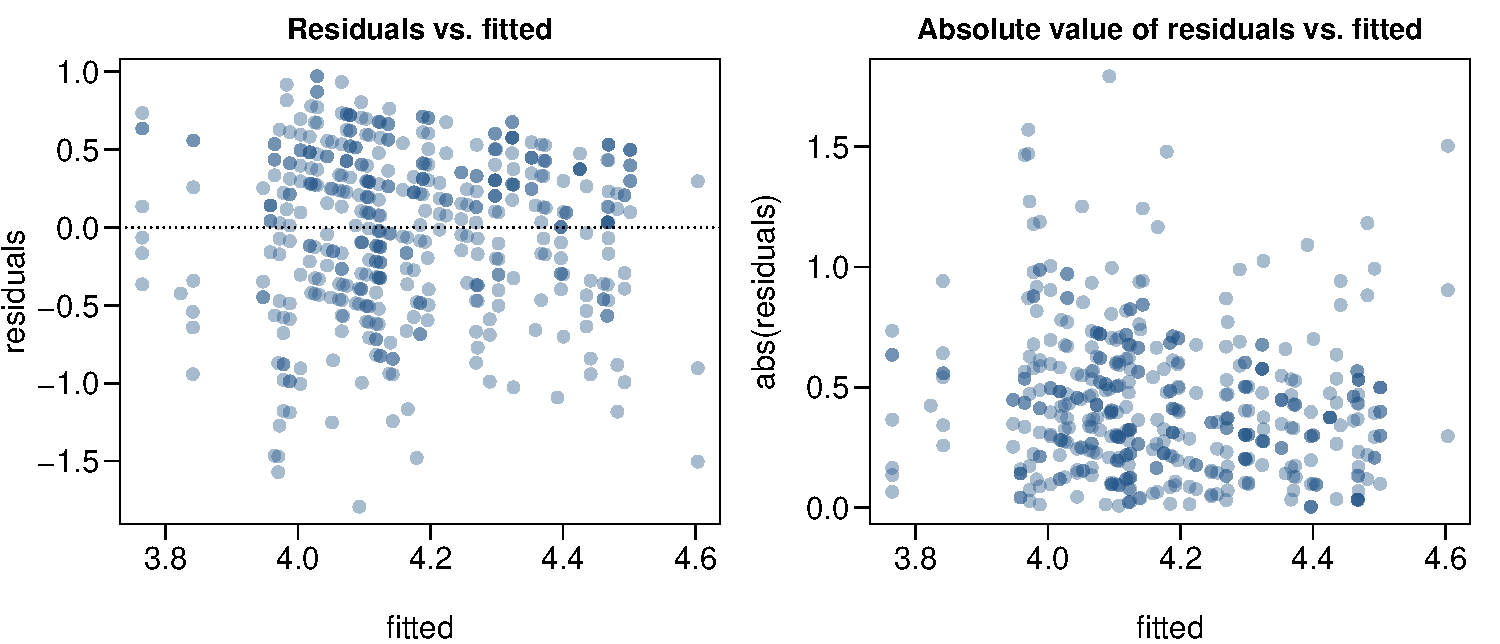
\includegraphics[width=\textwidth]{9-3_model_cond/figures/beauty/homo_res}
\end{center}

\dq{Does this condition appear to be satisfied?}

\end{frame}

%%%%%%%%%%%%%%%%%%%%%%%%%%%%%%%%%%

\begin{frame}
\frametitle{Checking constant variance - recap}

\begin{itemize}

\item When we did simple linear regression (one explanatory variable) we checked the constant variance condition using a plot of \hl{residuals vs. x}.

\item With multiple linear regression (2+ explanatory variables) we checked the constant variance condition using a plot of \hl{residuals vs. fitted}. 

\end{itemize}

$\:$ \\

\dq{Why are we using different plots?}

\soln{\only<2>{In multiple linear regression there are many explanatory variables, so a plot of residuals vs. one of them wouldn't give us the complete picture.
}}

\end{frame}

%%%%%%%%%%%%%%%%%%%%%%%%%%%%%%%%%%

\begin{frame}[fragile]
\frametitle{(3) independent residuals}

scatterplot of residuals vs. order of data collection: \\

\begin{center}
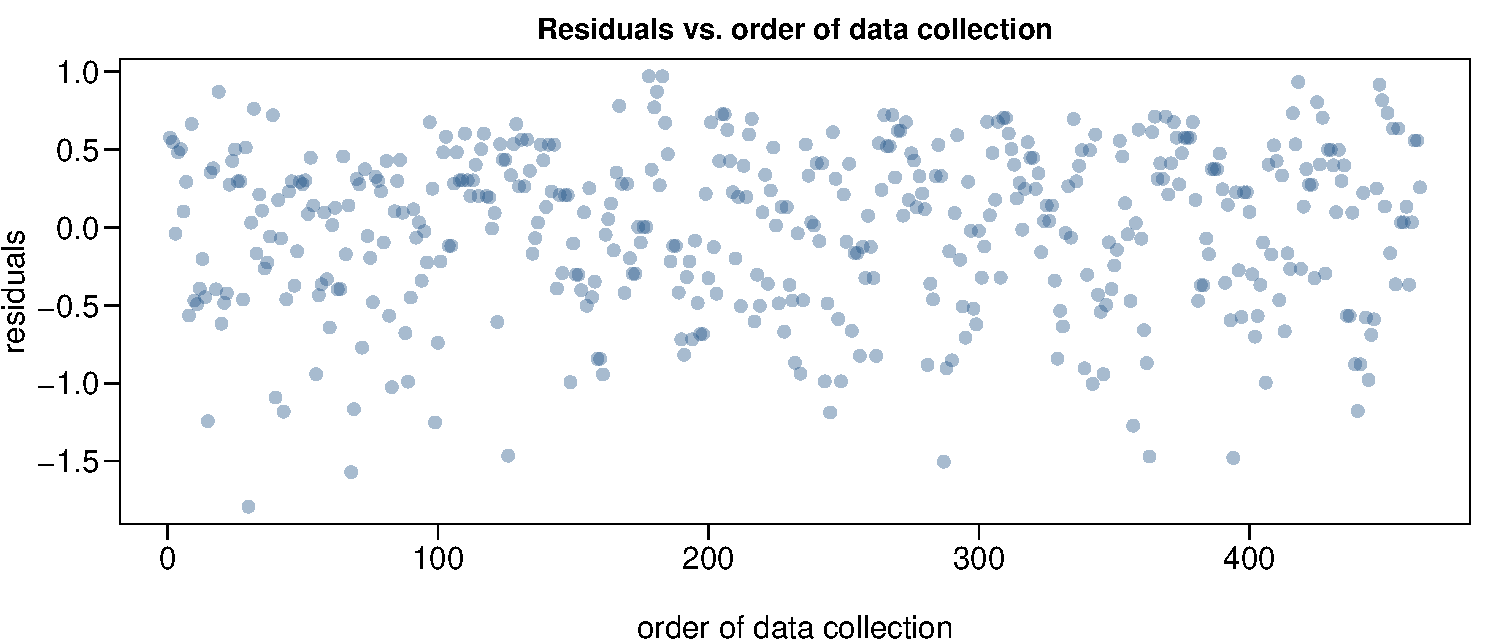
\includegraphics[width=0.8\textwidth]{9-3_model_cond/figures/beauty/indep_res}
\end{center}

\dq{Does this condition appear to be satisfied?}

\end{frame}

%%%%%%%%%%%%%%%%%%%%%%%%%%%%%%%%%%

\begin{frame}
\frametitle{More on the condition of independent residuals}

\begin{itemize}

\item Checking for independent residuals allows us to indirectly check for independent observations.

\item If observations and residuals are independent, we would not expect to see an increasing or decreasing trend in the scatterplot of residuals vs. order of data collection.

\item This condition is often violated when we have time series data. Such data require more advanced time series regression techniques for proper analysis.

\end{itemize}

\end{frame}

%%%%%%%%%%%%%%%%%%%%%%%%%%%%%%%%%%

\begin{frame}[fragile]
\frametitle{(4) linear relationships}

scatterplot of residuals vs. each (numerical) explanatory variable:

\begin{center}
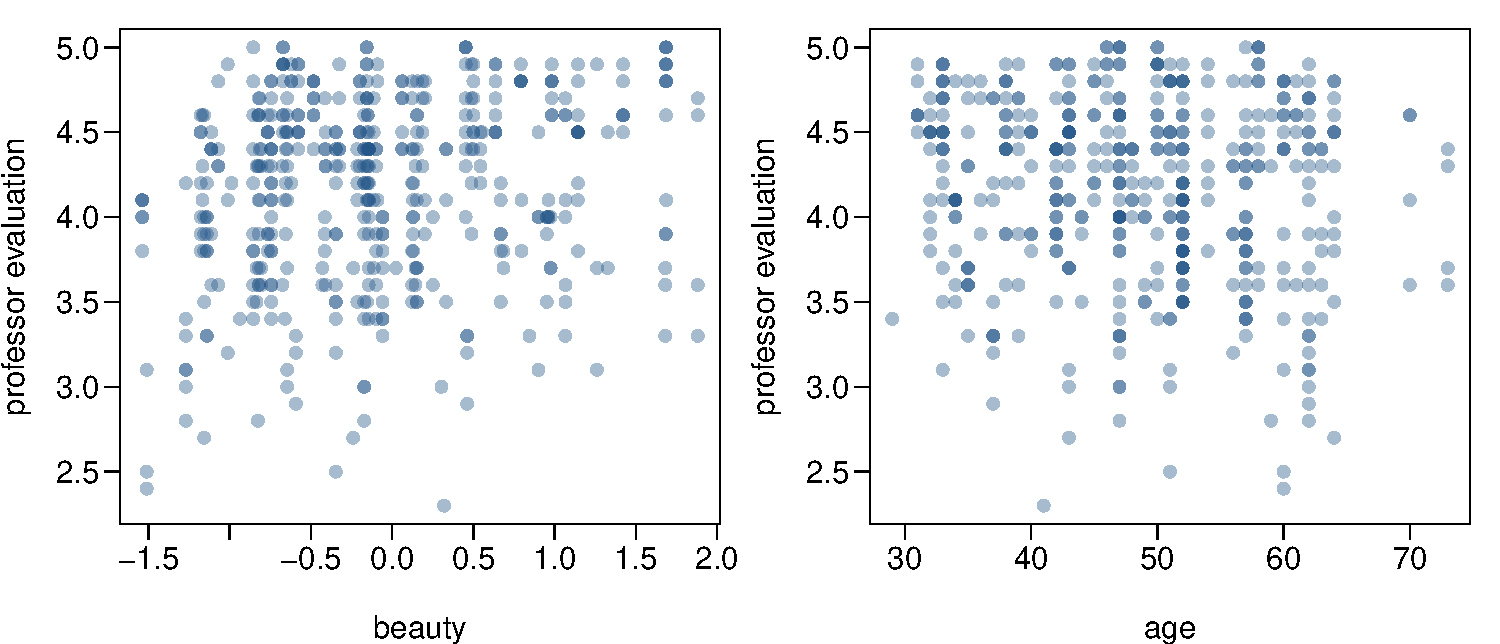
\includegraphics[width=0.8\textwidth]{9-3_model_cond/figures/beauty/linear}
\end{center}

\dq{Does this condition appear to be satisfied?}

\Note{We use residuals instead of the predictors on the y-axis so that we can still check for linearity without worrying about other possible violations like collinearity between the predictors.}

\end{frame}

%%%%%%%%%%%%%%%%%%%%%%%%%%%%%%%%%%%

\subsection{Options for improving the model fit}

%%%%%%%%%%%%%%%%%%%%%%%%%%%%%%%%%%%%

\begin{frame}
\frametitle{Several options for improving a model}

\begin{itemize}

\item Transforming variables
\item Seeking out additional variables to fill model gaps
\item Using more advanced methods that would account for challenges around inconsistent variability or nonlinear relationships between predictors and the outcome

\end{itemize}

\end{frame}

%%%%%%%%%%%%%%%%%%%%%%%%%%%%%%%%%%%%

\begin{frame}
\frametitle{Transformations}

If the concern with the model is non-linear relationships between the explanatory 
variable(s) and the response variable, transforming the response variable can be helpful. 

\begin{itemize}

\item Log transformation (log $y$)
\item Square root transformation ($\sqrt{y}$)
\item Inverse transformation ($1/y$)
\item Truncation (cap the max value possible)

\end{itemize}

It is also possible to apply transformations to the explanatory variable(s), however 
such transformations tend to make the model coefficients even harder to interpret.

\end{frame}

%%%%%%%%%%%%%%%%%%%%%%%%%%%%%%%%%%%%

\begin{frame}
\frametitle{Models can be wrong, but useful}

\begin{quote}
All models are wrong, but some are useful. - George Box
\end{quote}

\begin{itemize}

\item No model is perfect, but even imperfect models can be useful, as long as we are clear and report the model's shortcomings.

\item If conditions are grossly violated, we should not report the model results, but instead consider a new model, even if it means learning more statistical methods or hiring someone who can help.

\end{itemize}

\end{frame}

%%%%%%%%%%%%%%%%%%%%%%%%%%%%%%%%%%%%
%\input{9-4_mlr_case_study/9-4_mlr_case_study}
\input{9-5_logistic_reg/9-5_logistic_reg}


%%%%%%%%%%%%%%%%%%%%%%%%%%%%%%%%%%%%
% End document
%%%%%%%%%%%%%%%%%%%%%%%%%%%%%%%%%%%%

\end{document}